%!TEX root = ../Thesis.tex

\chapter{Anhang - Verwendete Datensätze}
\label{cha:anhang_a}

Nachfolgend sind Aufnahmen der in dieser Arbeit verwendeten Luftaufnahmen zu sehen.

\subsection*{Datensatz Entennest}

\begin{minipage}{0.55\textwidth}
    \begin{figure}[H]
        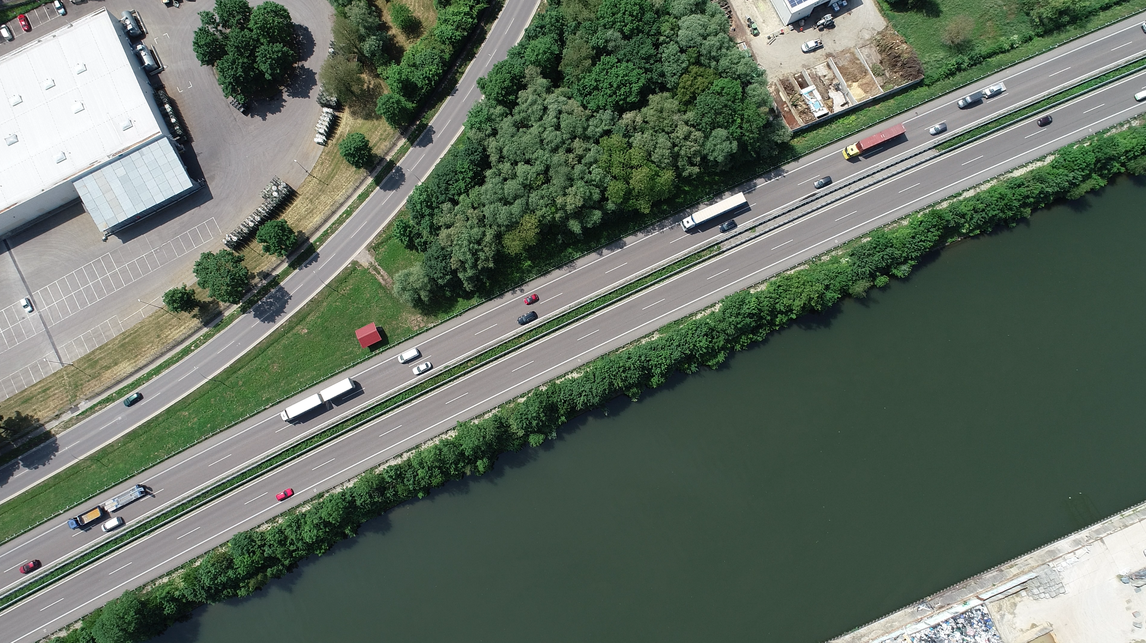
\includegraphics[width=\linewidth]{resources/img/Anhang/Entennest}
    \caption[]{Staßenabschnitt Aufnahme Entennest}
    \label{fig:anhang_ds_entennest}
    \end{figure}
\end{minipage} \hfill
\begin{minipage}{0.35\textwidth}
    \begin{tabular}{ll}
    \textbf{Anzahl Trajektorien}: &  224 \\
    \textbf{Anzahl Ziel-Fahrspuren}: & 6 \\
    \end{tabular}
\end{minipage}

\subsection*{Datensatz Neckartor}

\begin{minipage}{0.55\textwidth}
    \begin{figure}[H]
        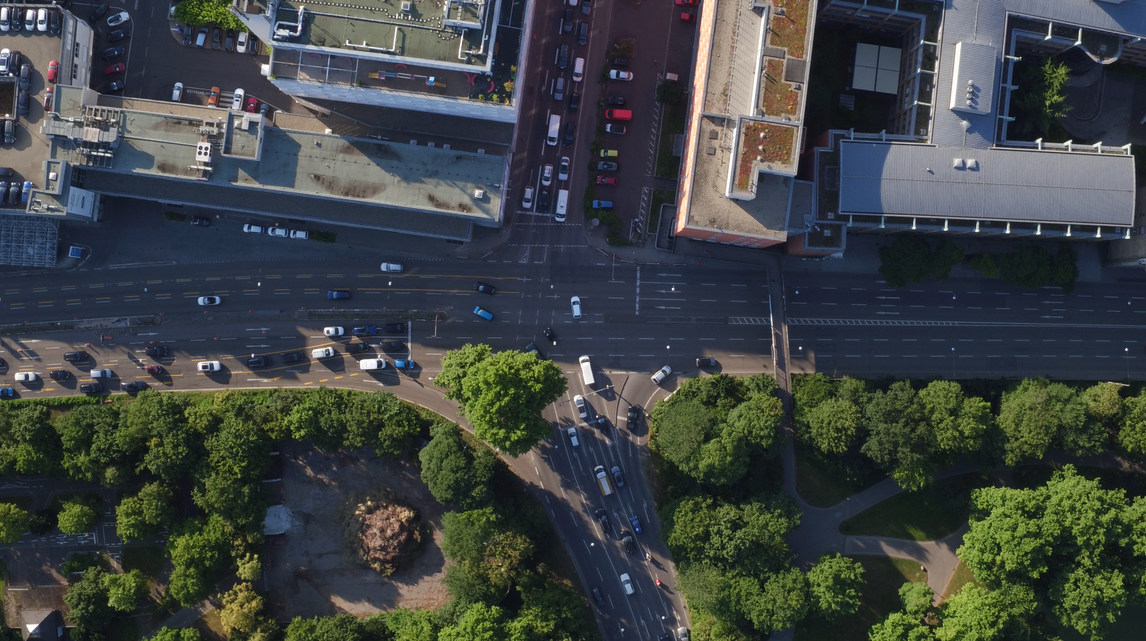
\includegraphics[width=\linewidth]{resources/img/Anhang/Neckartor}
    \caption[]{Staßenabschnitt Aufnahme Neckartor}
    \label{fig:anhang_ds_neckartor}
    \end{figure}
\end{minipage} \hfill
\begin{minipage}{0.35\textwidth}
    \begin{tabular}{ll}
    \textbf{Anzahl Trajektorien}: & 1240 \\
    \textbf{Anzahl Ziel-Fahrspuren}: & 14 \\
    \end{tabular}
\end{minipage}

\subsection*{Datensatz Heilbronner-Straße}

\begin{minipage}{0.55\textwidth}
    \begin{figure}[H]
        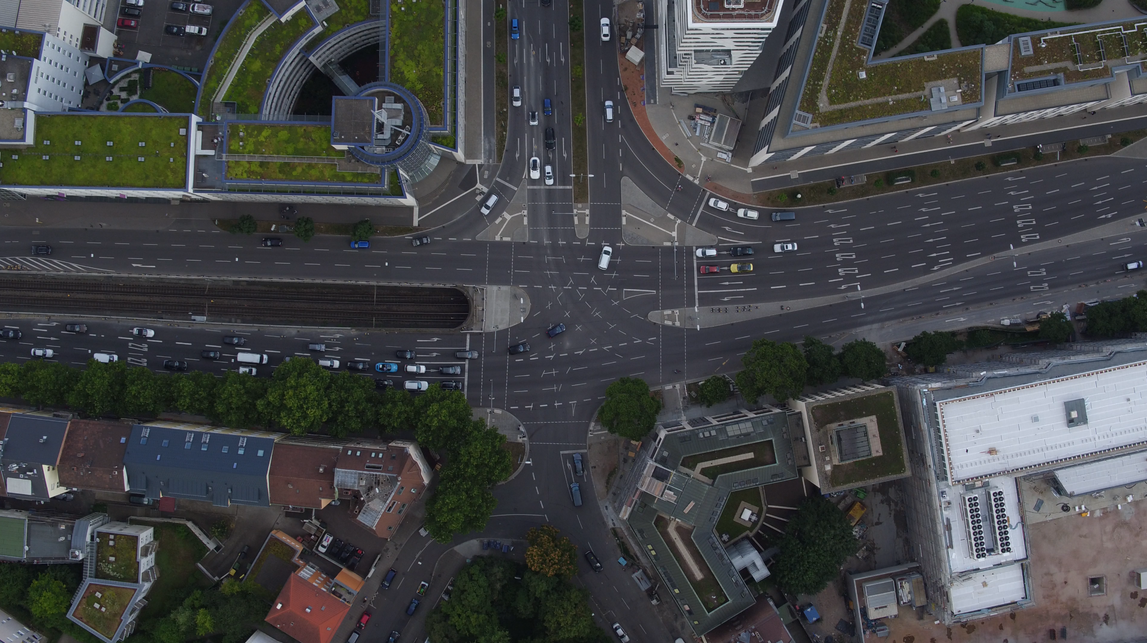
\includegraphics[width=\linewidth]{resources/img/Anhang/Heilbronner}
    \caption[]{Staßenabschnitt Aufnahme Heilbronner-Straße}
    \label{fig:anhang_ds_heilbronner}
    \end{figure}
\end{minipage} \hfill
\begin{minipage}{0.35\textwidth}
    \begin{tabular}{ll}
    \textbf{Anzahl Trajektorien}: &  1056 \\
    \textbf{Anzahl Ziel-Fahrspuren}: & 17 \\
    \end{tabular}
\end{minipage}

\subsection*{Datensatz Düsseldorf}

\begin{minipage}{0.55\textwidth}
    \begin{figure}[H]
        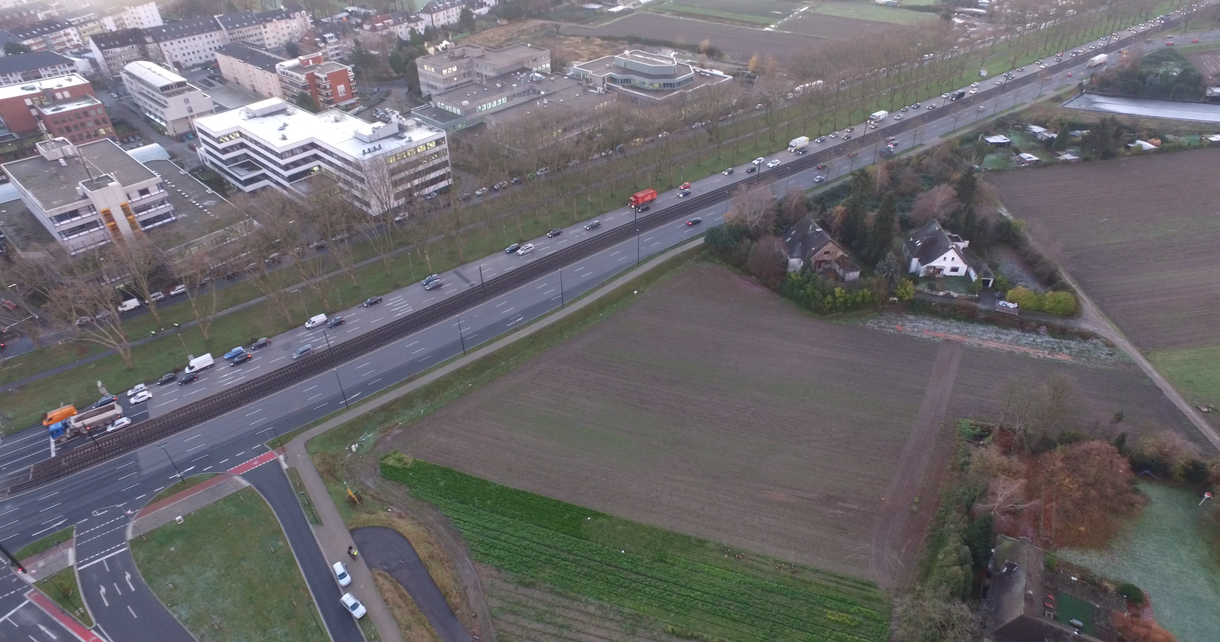
\includegraphics[width=\linewidth]{resources/img/Anhang/Duesseldorf}
    \caption[]{Staßenabschnitt Aufnahme Düsseldorf}
    \label{fig:anhang_ds_duesseldorf}
    \end{figure}
\end{minipage} \hfill
\begin{minipage}{0.35\textwidth}
    \begin{tabular}{ll}
    \textbf{Anzahl Trajektorien}: & 1705 \\
    \textbf{Anzahl Ziel-Fahrspuren}: & 10 \\
    \end{tabular}
\end{minipage}

\subsection*{Datensatz Steinheim}

\begin{minipage}{0.55\textwidth}
    \begin{figure}[H]
        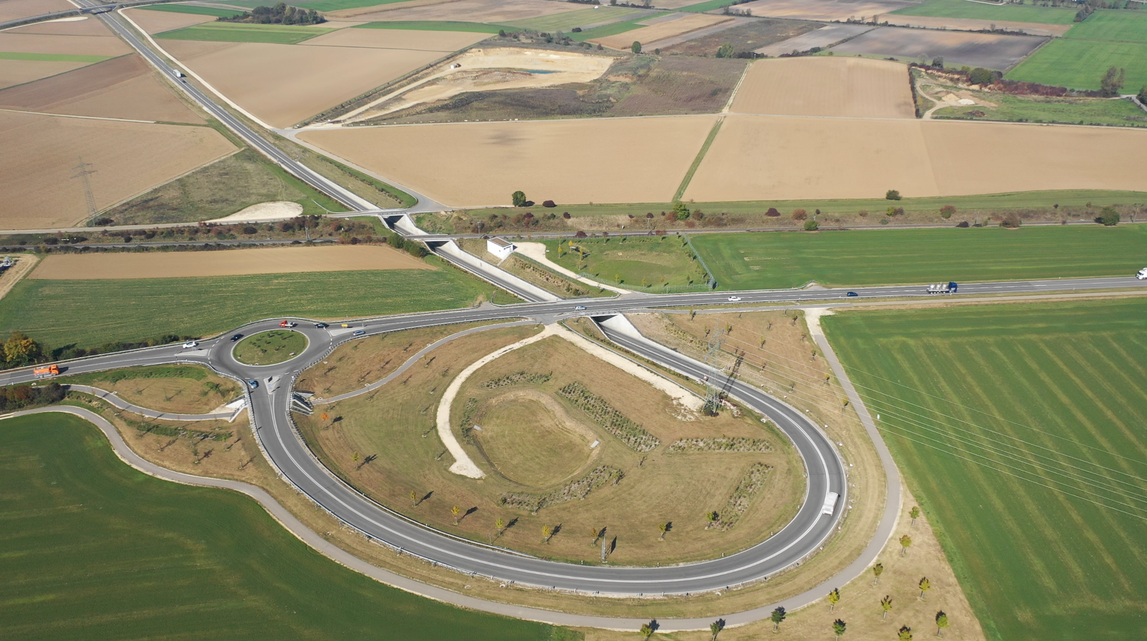
\includegraphics[width=\linewidth]{resources/img/Anhang/Steinheim}
    \caption[]{Staßenabschnitt Aufnahme Steinheim}
    \label{fig:anhang_ds_steinheim}
    \end{figure}
\end{minipage} \hfill
\begin{minipage}{0.35\textwidth}
    \begin{tabular}{ll}
    \textbf{Anzahl Trajektorien}: & 754 \\
    \textbf{Anzahl Ziel-Fahrspuren}: & 4 \\
    \end{tabular}
\end{minipage}